\documentclass[12pt,a4paper]{article}
\usepackage[left=1in, right=1in, top=1in, bottom=1in, footskip=.25in]{geometry}
\usepackage{natbib}

\usepackage{float}
\usepackage{rotating}
\usepackage{graphicx}
\graphicspath{ {../figures/} }
\usepackage{wrapfig}
\usepackage{changepage} 
\usepackage[table,xcdraw]{xcolor}
\usepackage{setspace}
\usepackage{gensymb}

\usepackage{caption}
\captionsetup[figure]{font=footnotesize}
\captionsetup[table]{font=footnotesize}

\usepackage[nottoc,numbib]{tocbibind} 
\settocbibname{References}

% for indending different levels
\newenvironment{indent1}[1][.5cm]{\begin{adjustwidth}{#1}{}}{\end{adjustwidth}}
\newenvironment{indent2}[1][1cm]{\begin{adjustwidth}{#1}{}}{\end{adjustwidth}}


% to make TOC link to document
\usepackage[hidelinks]{hyperref}
\hypersetup{
    colorlinks=true, %set true if you want colored links
    linktoc=all,     %set to all if you want both sections and subsections linked
    linkcolor=blue,  %choose some color if you want links to stand out
    citecolor=black,
    linktocpage=true, 
}
\usepackage[noabbrev]{cleveref}


\begin{document}




\begin{titlepage}
\begin{center}
\vspace*{7cm}
\begin{LARGE}
\textbf{Trends in Forest Ecology and Succession at Howland Forest}
\end{LARGE}

\vspace{6.5cm}

\begin{Large}
\textbf{Jamis M. Bruening, Ph.D. Student}\\
\end{Large}

\vspace*{0.5cm}


MnM4SDS Final Project Paper \\
Instructor: Dr. Taylor Oshan \\
Department of Geographical Sciences, \\
University of Maryland \\
\vspace*{.5cm}
\today 


\vspace*{5cm}

\end{center}
\end{titlepage}
\newpage

\setcounter{tocdepth}{2}
\tableofcontents
\newpage

\doublespacing

\section{Introduction}

\subsection{Background}

This project leverages a data set of tree locations and their associated physical attributes to identify and explain ecological trends related to forest succession at Howland Experimental Forest, located in central Maine.  Howland Forest (HF) is a secondary forest, meaning it was previously subject to some type of human land use, but at some point in the past that usage changed; the land was no longer `used' by humans and over time it returned to a more natural state \citep{hurtt2011}.  An example of this concept is a secondary forest that establishes and regrows on an abandoned agricultural field, as happened throughout New England in the early 20th century \cite{foster1998,canadell2007saturation}. This concept of secondary lands is central to my dissertation research.  Pioneered by UMD GEOG's Dr. George Hurtt, decades of work have shown that the rise of these secondary lands have contributed significantly to the global land carbon sink, and specifically in the northeast United States \citep{hurtt2002,hurtt2006,albani2006,houghton2012,houghton2017}.  

The worlds leading researchers in the global carbon cycle and terrestrial land fluxes argue that about two-thirds of the `missing carbon sink' (the portion of carbon missing from the atmosphere that cannot be accounted for in top-down global carbon budgeting and thus must have been fixed on the terrestrial land surface) is located in the mid-latitudes, due in large part to the regrowth of secondary forests from bare ground \citep{schimel2015,houghton2018}.  My dissertation research is focused on these secondary forested lands in the northeast United States, specifically the future carbon gain and trajectory of above-ground biomass accumulation with continued forest regrowth and natural secondary succession.  A central component to this area of study is the age distribution of all the trees in a forest, which is in turn coupled with the succession status and species composition of said forest.  As a tree ages it gets larger, and stores an increasing amount of carbon.  My interests are in using LiDAR to predict the age of a forest from information about its vertical and horizontal structure, and this estimate the future carbon gain through continued forest regrowth, across northern New England.  To do so, I need a better understanding of forest succession in forests characteristic in the region, and thus I have dedicated this project to interrogating a spatial ecological data set to identify trends in species distribution and forest succession at a site in central Maine.  Throughout this course I was exposed to various methods in spatial data science, and I have applied some of them here in an ecological context.  As much of the spatial data science community is directed towards answering spatial questions in different fields such as urban dynamics, econometrics, demography and geopolotics, there is substantial room for new applications of these methods in environmental and ecological contexts.  This project attempts identify and explain spatial trends in forest succession using cutting edge methods in spatial data science.  

\subsection{Objectives}

Over the course of the semester my project's objectives changed slightly as I worked through the analysis, encountered and addressed problems, and learned new methods.  Outlined here are my end-objectives, as were possible in a relatively short amount of time to perform the analysis.  When possible I have preserved the words verbatim from my initial project proposal.

\begin{enumerate}

\item Use exploratory techniques to identify spatial trends in ecological variables
\item Employ spatial data sciences methods to explain the presence and drivers to ecological trends
\item \textit{Determine the relationship between spatial ecological trends and additional environmental (site) variables, such as temperature, soil moisture, topography.}

\end{enumerate}

Number 3 is italicized because I did not have time to address it given the time constraints on the project.

\section{Literature Review}

I applied several methods of analysis from this course, based on the specifics of my project's data source and research questions.  Some methods and concepts I had been exposed to in previous courses, but I gained a better practical knowledge of them here.  The prime example is of spatial autocorrelation (or association), and specifically local indicators (LISA) \citep{anselin1995,symanzik2014exploratory}.  In two previous courses I've learned about spatial association, and the idea of spatial autocorrelation, however in this class I gained a deeper understanding and practical knowledge of the local indicators of these relationships.  In his seminal paper on the topic, \cite{anselin1995} essentially created the field of exploratory spatial data analysis and local spatial associations.  This work provided several novel and ground breaking methods to quantitatively assess the extent to which spatial associations exist with a spatial data set, a numerical way to represent Tobler's first Law of Geography.  These methods have are used to identify the extent to which `hotspots' of nonstationarity exist, a measure of how similar a value at one location is to over nearby observations, and the extent to which spatial position influences relationships between processes or variables.  

Continuing in this vein and at around the same time, \cite{brunsdon1996geographically} developed a method of exploring nonstationarity through what they termed as geographically weighted regression (GWR).  This method addressed a prominent issue in quantitative geography at the time, that in many instances, a `global' set of relationships that is the identified through aspatial methods may not hold true across and throughout space.  This new GWR technique assumes that spatial position is integral to the process being studied, and the relationship between variables may not hold true everywhere throughout the study area.  They thus developed a type of linear regression model that accounts for the spatial position of observations, and fits a set of local models for each observation.  This technique allows for different coefficients for variables for each observation, thus allowing the model to pick up on spatial variations between response and predictors that a regular, global regression model inherently cannot.  

These methods have been further developed over the past 2+ decades, with new implementations of these concepts for different processing systems or scripting languages, as well as the addition of new functionality and methods.  Multiscale Geographically Weighted Regression (MGWR) is one such example \citep{fotheringham2017multiscale,oshan2019mgwr}.  This method builds on the concepts of GWR, but even further reduces some of the spatial modeling assumptions.  Similar to how GWR rejects the assumption that a single relationship must hold true across a study area or region and allows for different model coefficients based on local regression fits, MGWR does not assume that the relationships between each predictor-response variable pair operates on the same spatial scale.  This method allows for spatial nonstationarity in the same way that GWR does, but also lets each predictor variable's spatial domain vary relative to the other predictor variables \citep{fotheringham2017multiscale}.

\subsection{Ecological basis for methods chosen}\label{eco_lit}

I chose these above methods based on my understanding of the landscape scale processes that drive ecological succession, and an understanding that the environmental variables that influence tree growth and succession may have different spatial scales on which they operate.  For example, gap regeneration theory and shade tolerance are foundational pillars of forest succession theory \citep{runkle1981gap,shugart1984theory,yamamoto1992gap}.  Yet it is also known that growing season climate and edaphic conditions are also crucially important to understanding forest growth and large scale ecological succession \citep{west2012forest}.  A baseline knowledge of landscape ecology necessitates that these processes must operate on extremely different spatial scales, from the very local, regarding gap theory and shade tolerance, to site-based and even regional scales for climate and soil characteristics.  Thus I wanted to incorporate methods that allowed for the spatial variation of relationships between individual tree canopy position and the physiological and environmental characteristics of this site.


\section{Data}\label{data}

The dataset I used represents every single live tree in the NASA Plot at HF.  The NASA plot is a 200 meter by 150 meter plot within HF established in 1989 for long term ecological monitoring.  Thus, the spatial positions of every single tree were mapped, and have been periodically updated as new trees establish and old trees experience mortality.  I was not looking at temporal trends in this analysis, so I subset the NASA Plot data to include only live trees at the most recent update in 2015, as well as only the most recent tree attributes measured in 2015.  My resultant data frame includes all trees with a diameter at breast height (DBH) greater than 5 cm within the plot, the coordinate locations of each tree, along with various physical attributes.  These include the DBH, tree height, distance between the base and the live crown, and its canopy class, which is a proxy for its successional status.  This variable is the dependent variable in my analysis, and is my primary interest in this project.  It is technically an ordinal variable, meaning it is a categorical variable in which the categories are ordered, and describes the position of the tree and its canopy in the forest relative to the neighboring trees.  There are six levels to this variable;  1: Super dominant, 2: Dominant, 3: Co-dominant, 4: Intermediate, 5: Overtopped, 6: Suppressed.  However, in ecology nothing is cleanly separated into distinct bins, so I've relaxed the assumption that this is a strict ordinal variable and have treated it as a continuous variable to be able to use many of the methods we learned in class.  I can justify this, because everything is a gradient in ecology, and almost never are complex organisms such as trees naturally separated into rigid classes based on their physical properties.  For example, two trees could both be super-dominant, meaning their canopies extent up beyond most other neighboring trees, yet one could be slightly taller than the other and receive slightly more sunlight than the other.  In this case while they are both classified as super dominant, one is still more super-dominant than the other.  Thus, I treat the canopy position variable as continuous based on this rationale, and I do not expect this choice to have substantially impacted my results or violated any other assumptions downstream in my analysis.

\section{Methods}

\subsection{Plotting and spatial visualization of variables}

My first approach was to plot the tree locations in 2-dimensional space, adding a third and fourth dimension to visualize my dependent and independent variables at the same time, using colors and graduated symbol sizes to represent the physical tree attributes.  The Seaborn module is extremely functional for this, and allowed me to produce maps that gave me a very useful visualization of the complex picture of the ecological succession at HF  Adding a third and fourth dimension to the spatial plots of the tree locations was especially helpful to start visually identifying spatial trends in these variables, and informed my methods selection later in explicitly quantifying these complex spatial differences.  See \cref{figures} for all plots.  I chose to put all figures in a separate section at the end to allow for large figure sizes.  If I included the figures in-text, I would need to shrink many of them which would reduce their readability.  Each plot will also be linked to individually when referenced in the results or discussion section.  

Following regular data analysis procedures, I also produced aspatial plots, both in this preliminary exploratory stage to identify aspatial trends in my dependent and independent variables, but also in interpreting the results of the variables models run later in the analysis.  Plotting residuals in space and also by canopy type was crucial to my analysis, and provided my initial motivation to include a spatial fixed effect model. 

\subsection{Exploratory modeling of successional status}

In plotting the spatial locations of the trees and their associated physical attributes, it became apparent that there was a high degree of something I call ecological noise (this is a non-technical term).  Ecology is complex and messy, and sometimes an effective technique to reduce this noise and identify underlying processes or trends is to slightly aggregate data to visually identify a signal that is present.  Thus, I delineated a 5 meter by 5 meter grid, overlaid on the NASA plot, to use both to segment the plot into regularly sized areas, and to aggregate the attributes of the trees within each gird cell to smooth out the `ecological noise'.  The size of the grid here is important; too large a grid cell and I will start to smooth out an underlying signal, and too small a grid cell and I will not reduce any noise and have many grid cells without any trees in them.  This is a somewhat arbitrary decision, based in part on my intuition and moderate knowledge of forested systems.  In a maturing forest, a 25 meter squared area may have a handful of trees, depending on their size and succession status, and this would be enough to reduce the noise levels present in the individual trees and bring out any underlying ecological signals present.  To help represent the ecological characteristics of the NASA plot at this new resolution of 5 meters, I aggregated the physical tree attribute data at this resolution, as well as calculated several additional ecological variables for each 5 meter grid cell in the plot.  The resultant gridded variables are as follows:

\begin{itemize}
\item Average height, average diameter (mean of all trees in cell)
\item Mode successional status (most common successional status of all trees in cell)
\item Species richness (number of different tree species in each cell)
\item Tree density (total number of trees in each cell)
\item Heterogeneity Index (species richness divided by total number of species)
\end{itemize}

With the plotting and data munging completed, I transitioned to some initial, basic modeling.  I ran a set of two initial models, an aspatial OLS model and an OLS with spatial fixed effects by including the gridded transect variable as a grouping variable.  In both models (and all others in the analysis) my dependent variable is the canopy position of each tree,  and the independent tree-attribute variables are tree diameter (DBH), height (HT), and distance between the base and live crown (BLC), explained above in \cref{data}.   I chose this initial two-model approach because it allowed me to partition the influence of aspatial physical attributes of the tree and the spatial component of ecological succession.  By comparing the results between these two models, I was able to identify the presence of a spatial trend in addition to the explanatory power of both DBH and HT in the successional status of each tree.  These models were run at the individual tree level, with the gridded transect variable added to represent space in the fixed effects model.

\subsection{ESDA and GWR}

Following the spatial fixed model, I ran a LISA analysis on each of the main variables in my study, aggregated at the 5 meter grid level, as well as several other variables I calculated to help represent the characteristics of the NASA plot at the new resolution of 5 meters.  I used queen contiguity weights, a decision that was again informed by ecological theory.  There is no \textit{a priori} distance at which ecological processes operate in a forest, and arguably different processes happen at different scales (see \cref{eco_lit}), so this eliminated a distance-based weights matrix.  In the choices of contiguity based weights, queen weights make the most sense ecologically.  The square grid I generated has now ecological basis other than an arbitrary way to segment my plot into smaller regions.  There is no ecological process that happens in orthogonal space (rook or bishop based weights); the most appropriate scheme is to consider all neighboring areas similarly examining ecological trends, thus necessitating a queen contiguity based weighting scheme.

For each variable (physical tree-attributes such as DBH and HT and locale-specific attributes such as species richness or tree density) I ran a LISA plot analysis to identify patterns of spatial dependence on the variables.  My rationale for doing this was to explore the potential for any of these variables to match the effect that seen in the spatial fixed effects model, in addition to better understand the spatial-ecological trends in each independent variable, and how these may relate to the ecological succession of the trees in the NASA plot.  I tested the significance of Moran's I for each variable, and plotted each variable in space aggregated at the 5 meter grid level.

In a further attempt to assess the extent to which any of my tree or grid level variables capture the effects of the grid variable seen in the spatial fixed effects model, I ran both a GWR and MGWR.  The rationale for this step was that I could envision a scenario where the drivers of succession vary based on the location within a forest.  Land-use history is such an important driver of ecological succession, and I do not have any variables that provide any such information.  If part of this plot was disturbed more recently than another, the effects on the successional status of the trees there would almost certainly be present, and not captured under the assumption that the relationship between the independent variables and crown positions the same regardless of position within the plot.  

\section{Results}

In the aspatial OLS model, DBH and HT explained roughly 50\% of the variation in canopy class ($R^{2} = 0.54, p_{dbh} = 0.00, p_{ht} = 0.00, p_{intercept} = 0.00$).  The intercept term is 6.2, indicating that when HT and DBH are = 0, the successional status of the tree is at the lowest level, as would be expected.  Here, and in other models, BLC has little-no effect and is not significant, and thus has been largely excluded from the rest of my interpretation and discussion.  The spatial fixed effect model explains almost an additional 30\% of the variation in canopy type ($R^{2} = 0.80, p_{dbh} = 0.00, p_{ht} = 0.00$).  A particularly interesting result from this model is the variation and significance of the intercept terms for each grid cell.  While similar to the regular OLS, the intercept terms to fluctuate between 4-7, indicating spatial heterogeneity in canopy type in the absence of the effects of DBH and HT.  This can be seen in mapping the residuals of both the OLS and spatial fixed effects models \cref{OLS_mod_residuals_map,SFE_mod_residuals_map}.  The OLS residuals have large, positive, significant spatial autocorrelation (I = 0.25, p = 0.001), while the spatial fixed model has a much lower level of negative spatial autocorrelation (I = -0.08, p = 0.001).  Visually, there is a clear spatial trend in the OLS residuals, while there is little or no obvious trend in the spatial fixed effect models residuals.  Interestingly, both models more accurately predict the successional status of more mature trees than those earlier on in the successional trajectory, indicating more variance in the physical attributes of younger trees than more older, established individuals (\cref{OLS_mod_residuals_by_Canopy,SFE_mod_residuals_by_Canopy}).  

The two variables with the largest spatial autocorrelation at the 5 meter grid cell level were tree density (I = 0.367, p = 0.001) and height (I = 0.356, p = 0.001), followed by the  heterogeneity index (I = 0.249, p = 0.001), diameter (I = 0.199, p = 0.001), and species richness (I = 0.172, p = 0.001).  Mode successional status had a relatively low value (I = 0.083, p = 0.001), which isn't surprising given that it is more difficult to meaningfully aggregate ordinal variables than continuous variables.  Due to this, I was not able to get any meaningful information from any modeling exercise performed at the grid cell level.  It seems that the mode successional status of all trees in a 5 meter grid cell isn't as meaningful an ecological attribute as considering the status of each tree individually. 

The geographically weighted regression shows a similar picture to the aspatial OLS module, when comparing the GWR's intercept term to the residuals in the aspatial OLS.  When variables are standardized, trends in the intercept term of a GWR typically indicate a process or set of processes that have not been captured by the variables in the model.  Similarly, in OLS when the residuals have a spatial pattern, it indicates the absence of a variable in the model that explains the trend.  To quantify the similarities between these two approaches, I ran a linear model predicting the OLS residual as a function of the GWR intercept term, stratified by tree canopy type \cref{ModelComparison_Cnpy1,ModelComparison_Cnpy2,ModelComparison_Cnpy3,ModelComparison_Cnpy4,ModelComparison_Cnpy5,ModelComparison_Cnpy6}.

\section{Discussion and Conclusions}

Ecology is both inherently aspatial and spatial, and the spatial processes operate at various scales.  This has been demonstrated through the two modeling exercised in this project, which both point to similar trends in forest succession as a function of physical tree characteristics (aspatial) and presumably site-related characteristics not represented by variables explicitly in these models, but identified by the intercept terms in both the spatial fixed effects and geographically weighted regressions.  A logical next step in this analysis is to include site-related environmental variables that can account for the spatial variation in these intercept terms in these models.  There are several that come to mind, mainly edaphic characteristics, as well as climatic variables such as localized average temperatures, soil moisture, all of which are influenced to varying degrees by the local topography.  It is well known that different tree species prefer different types of soil and climatic growing conditions; the same species growing on two different soil types may experience different growth trajectories, and tree successional status is both limited on poor growing sites and enhanced in favorable ones.  Thus, providing site-characteristics that are directly related to a tree's ability to grow healthily and compete with neighboring trees may very well help to explain the spatial trends not accounted for in this analysis thus far.

Modeling the successional status of trees is best done at the individual tree level.  While aggregating some tree and forest attributes to a grid may help visualization of ecological trends across a forest landscape, there is little information to be gained when looking at a composite measure of succession.  This is likely due to several factors that have to do with successional processes.  There are two main mechanisms by which trees reach maturity in an already established forest such as HF (there are more than only two but for the purposes of this paper I'm focusing on the two primary mechanisms that are most relevant here).  The first is that when a large tree falls over, it creates a gap in the canopy.  This gap is quickly filled by fast growing, intermediate shade tolerant trees.  These individuals out compete their slower growing neighbors and quickly fill the gap.  While it may take years to reach full maturity and peak successional status of a dominant or super dominant tree, there can easily be trees that comprise of different diameters and heights and even canopy levels growing in close proximity, as a function of the spatiotemporal dynamics of gap openings and closing throughout a relatively small forested area.  Conversely, shade tolerant trees can establish and begin maturing in a very shaded understory.  When a neighboring tree falls and creates a partial gap, these slower growing trees are poised to fill its place quicker than the faster growing trees because they've had a head start and have less growing to do to close and fill the gap than the intermediate shade tolerant trees that can only start growing once the gap opens and enough light penetrates through the canopy to the ground.  Both these processes mean that it is very common to have trees of very different successional stages, sizes, and heights in close proximity to one another, and thus an aggregate measure of the successional status of an area is probably less useful than looking at the individuals.  This analysis shows the complexity of succession in a forest, which is influenced by many different factors that vary at different rates in both time and space.  

This project has provided an initial picture of the site-specific characteristics of forest succession at HF, as well as several potential avenues for further research.  It is obvious from both theoretical and quantitative perspectives that nonstaionarity exists in the drivers of ecological succession at HF, and I'd like to provide a better identification of the spatial process that is captured in the GWR intercept term.  Further work should also probably include species-specific approaches, or segmenting species by their shade tolerance, as the relative proportions of the three shade tolerances (tolerant, intermediate, and intolerant) is also important for the successional trajectory of that forest and what mechanisms might be at play (environmental factors vs light availability and gap regeneration, for example).  This work provides an interesting application of spatial data science methods for assessing a well studied ecological phenomena which may be useful for further research in forest succession.



\newpage
\section{Figures}\label{figures}

\subsection{Exploratory Plotting}

%% BOXPLOT
\begin{figure}[H]
\centering
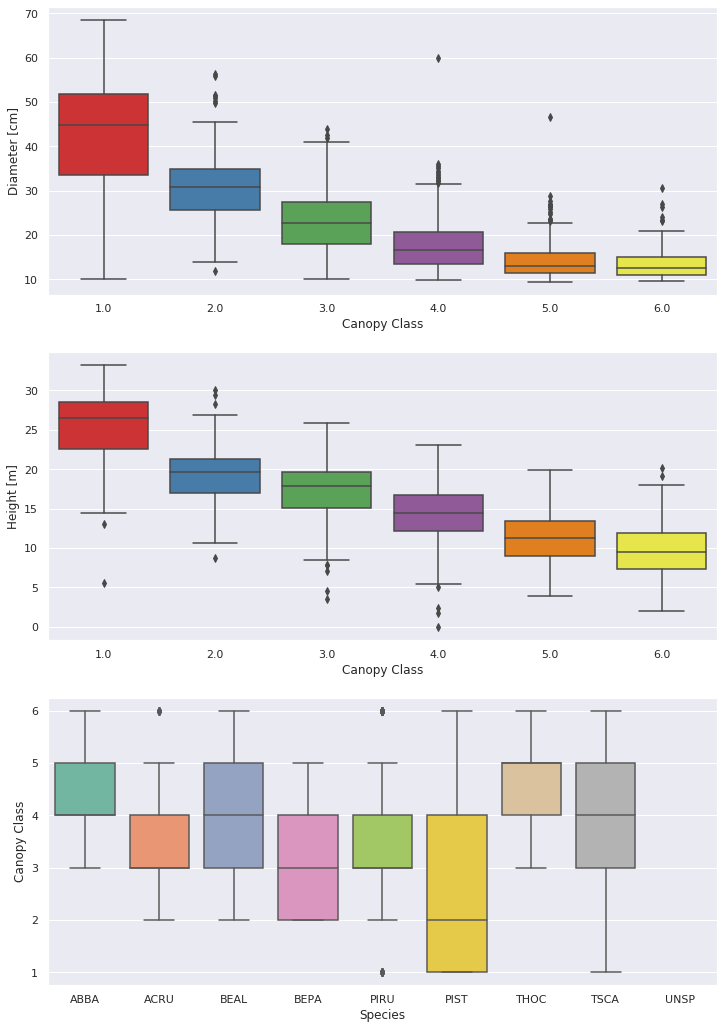
\includegraphics[scale=.55]{../figures/Eplot_Boxplot_Cnpy_vs_Height&DBH.png}
\caption{Boxplots of the dependent variable canopy class vs tree diameter (top), tree height (middle), as well as canopy class distributions by species (bottom).}
\label{Eplot_Boxplot_Cnpy_vs_Height&DBH} 
\end{figure}

%% SCATTER
\begin{sidewaysfigure}
\begin{figure}[H]
\centering
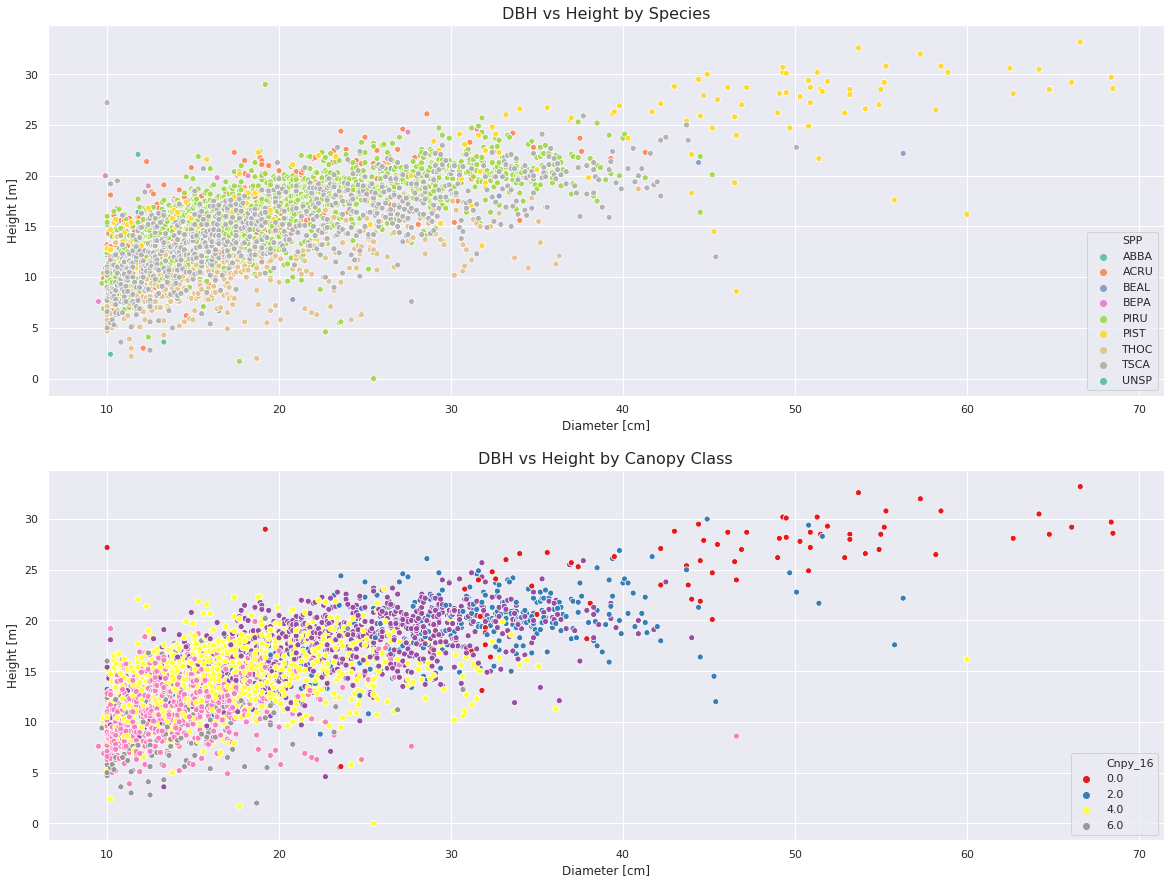
\includegraphics[scale=.55]{../figures/Eplot_Scatter_Height_vs_DBH_by_Cnpy&Species.png}
\caption{Scatter plots of tree diameter vs height, showing variations within species (top) and canopy class (bottom).}
\label{Eplot_Scatter_Height_vs_DBH_by_Cnpy&Species} 
\end{figure}
\end{sidewaysfigure}

%% TREEMAP
\begin{sidewaysfigure}
\begin{figure}[H]
\centering
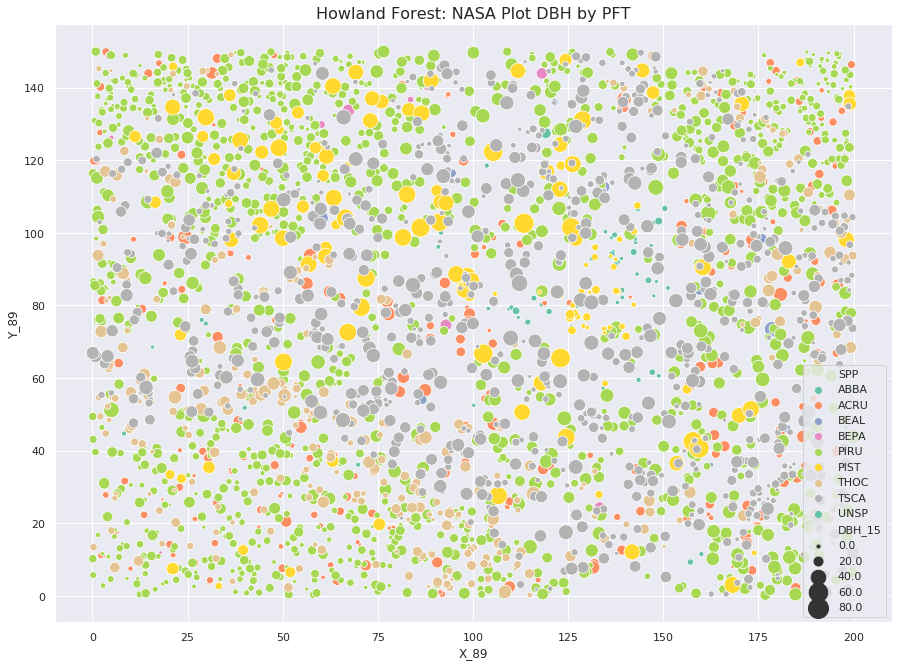
\includegraphics[scale=.75]{../figures/Eplot_TreeMap_bySpecies_byDBH.png}
\caption{Spatial position of each tree within the NASA plot, colored by species and sized by tree diameter.}
\label{Eplot_TreeMap_bySpecies_byDBH} 
\end{figure}
\end{sidewaysfigure}

%% TREEMAP
\begin{sidewaysfigure}
\begin{figure}[H]
\centering
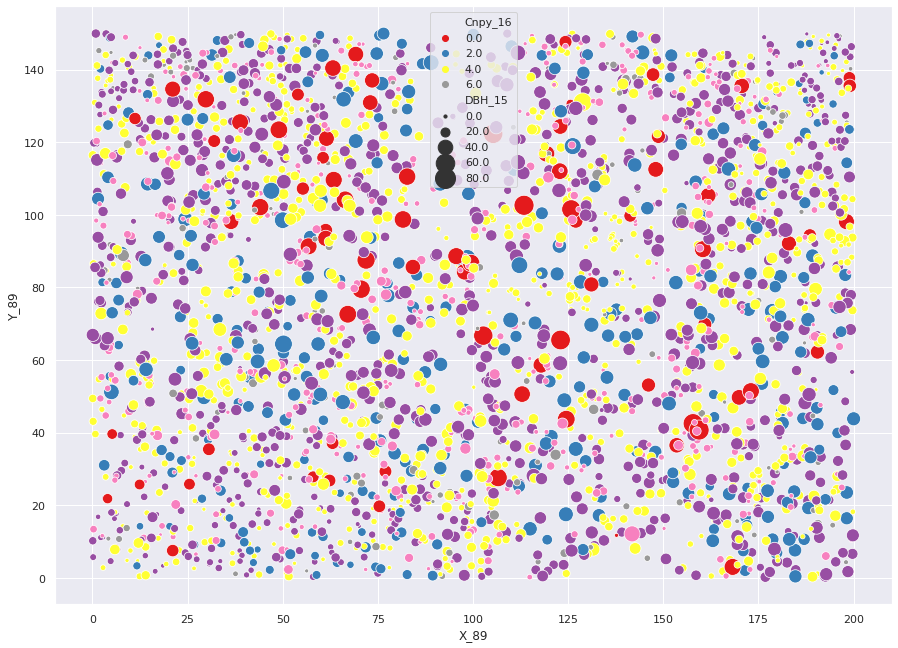
\includegraphics[scale=.75]{../figures/Eplot_TreeMap_byCnpy_byDBH.png}
\caption{Spatial position of each tree within the NASA plot, colored by canopy class and sized by tree diameter.}
\label{Eplot_TreeMap_byCnpy_byDBH} 
\end{figure}
\end{sidewaysfigure}








%%%%%%%%%%%%%%%%%%%%%%%%%%%%%%%%%%%%%%%%%%%%%%%%%%%
%%%%%%%%%%%%%%%%%%%%%%%%%%%%%%%%%%%%%%%%%%%%%%%%%%%
\newpage
\subsection{OLS and Fixed Effects Regression}

%% OLS MOD RESIDUALS MAP
\begin{figure}[H]
\centering
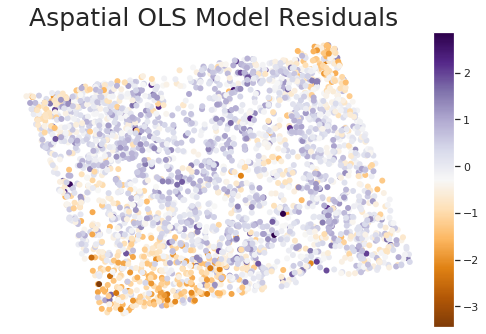
\includegraphics[scale=.8]{../figures/OLS_mod_residuals_map.png}
\caption{Spatial position of the trees within the NASA plot, colored by the residuals of the aspatial OLS model.}
\label{OLS_mod_residuals_map} 
\end{figure}

%% OLS MOD RESIDUALS BOXPLOT
\begin{figure}[H]
\centering
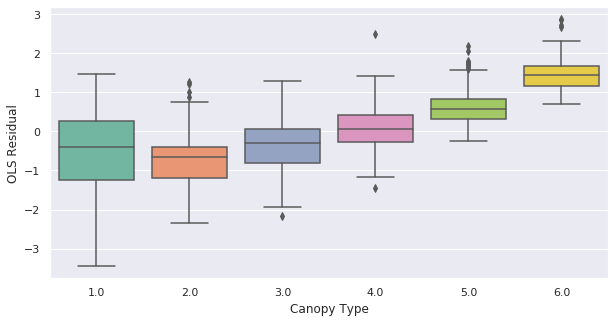
\includegraphics[scale=.7]{../figures/OLS_mod_residuals_by_Canopy.png}
\caption{Boxplot indicating the distribution of the aspatial OLS residuals by canopy class.  Notice the increasing trend, indicating the s spatial model misses some trend relating to canopy class of the younger, less mature trees (higher canopy class values).}
\label{OLS_mod_residuals_by_Canopy} 
\end{figure}


%% SFE MOD RESIDUALS MAP
\begin{figure}[H]
\centering
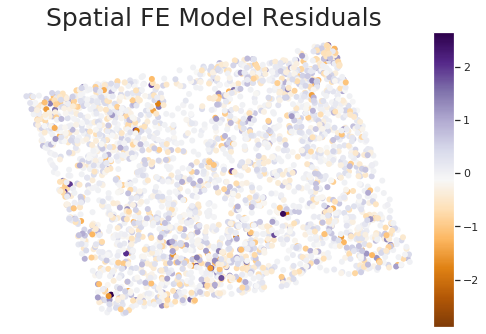
\includegraphics[scale=.8]{../figures/SFE_mod_residuals_map.png}
\caption{Spatial position of the trees within the NASA plot, colored by the residuals of the spatial fixed effects OLS model.}
\label{SFE_mod_residuals_map} 
\end{figure}

%% SFE MOD RESIDUALS BOXPLOT
\begin{figure}[H]
\centering
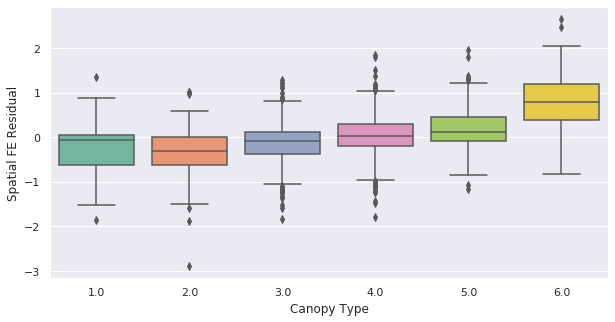
\includegraphics[scale=.7]{../figures/SFE_mod_residuals_by_Canopy.png}
\caption{Boxplot indicating the distribution of the spatial fixed effects OLS residuals by canopy class.  Notice the increasing trend is still present here, but must less pronounced than in the aspatial model, indicating a both spatial and aspatial component of the residuals in the OLS models.}
\label{SFE_mod_residuals_by_Canopy} 
\end{figure}

%%%%%%%%%%%%%%%%%%%%%%%%%%%%%%%%%%%%%%%%%%%%%%%%%%%
%%%%%%%%%%%%%%%%%%%%%%%%%%%%%%%%%%%%%%%%%%%%%%%%%%%

\subsection{ESDA}

%% ESDA HEIGHT
\begin{figure}[H]
\centering
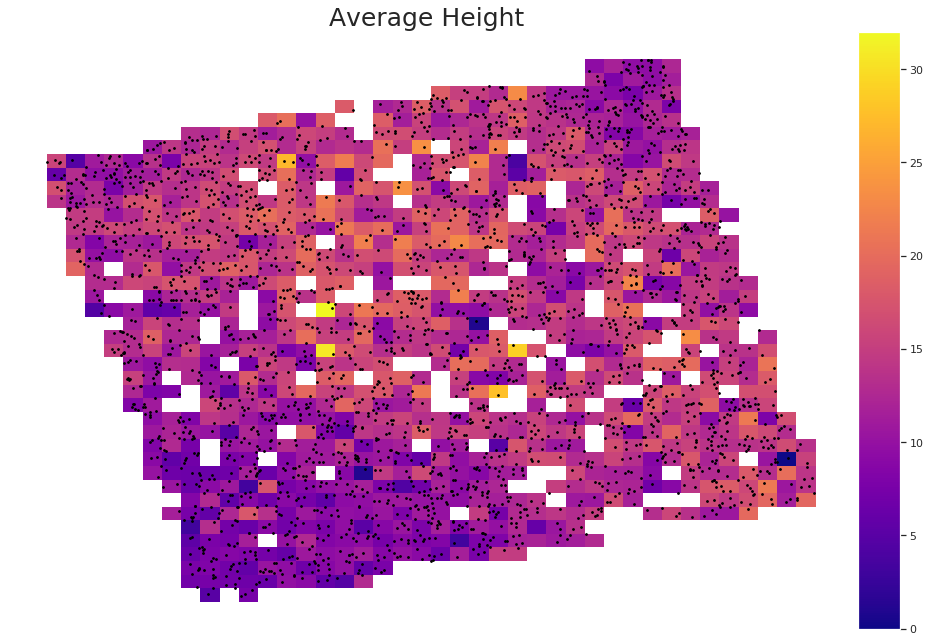
\includegraphics[scale=.45]{../figures/ESDA_height.png}
\caption{Gridded plot of average tree height at the 5 meter scale.}
\label{ESDA_height} 
\end{figure}

%% ESDA DBH
\begin{figure}[H]
\centering
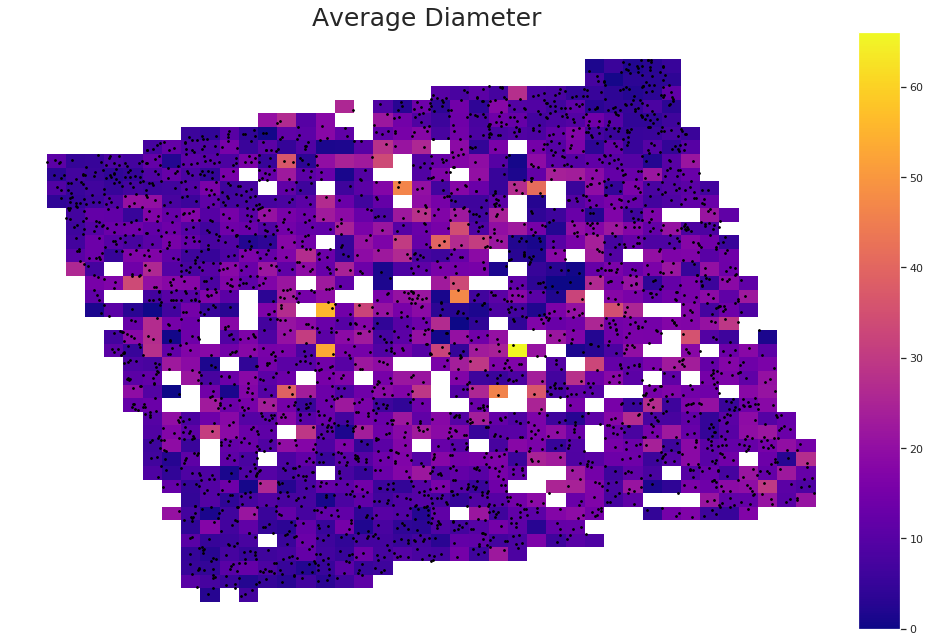
\includegraphics[scale=.45]{../figures/ESDA_dbh.png}
\caption{Gridded plot of average tree diameter at the 5 meter scale.}
\label{ESDA_dbh} 
\end{figure}

%% ESDA HEIGHT
\begin{figure}[H]
\centering
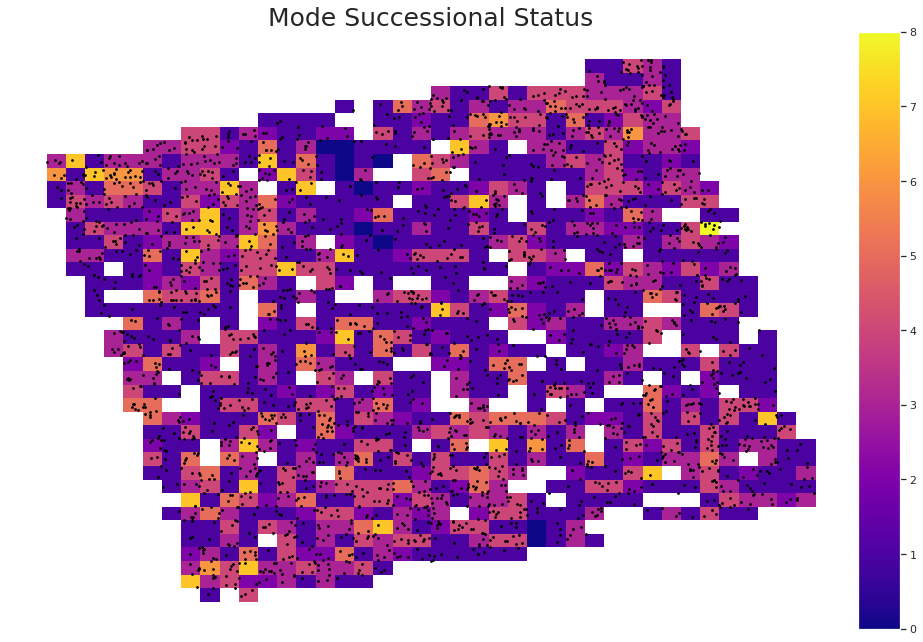
\includegraphics[scale=.45]{../figures/ESDA_cnpy.png}
\caption{Gridded plot of mode canopy class at the 5 meter scale.}
\label{ESDA_cnpy} 
\end{figure}

%% ESDA DBH
\begin{figure}[H]
\centering
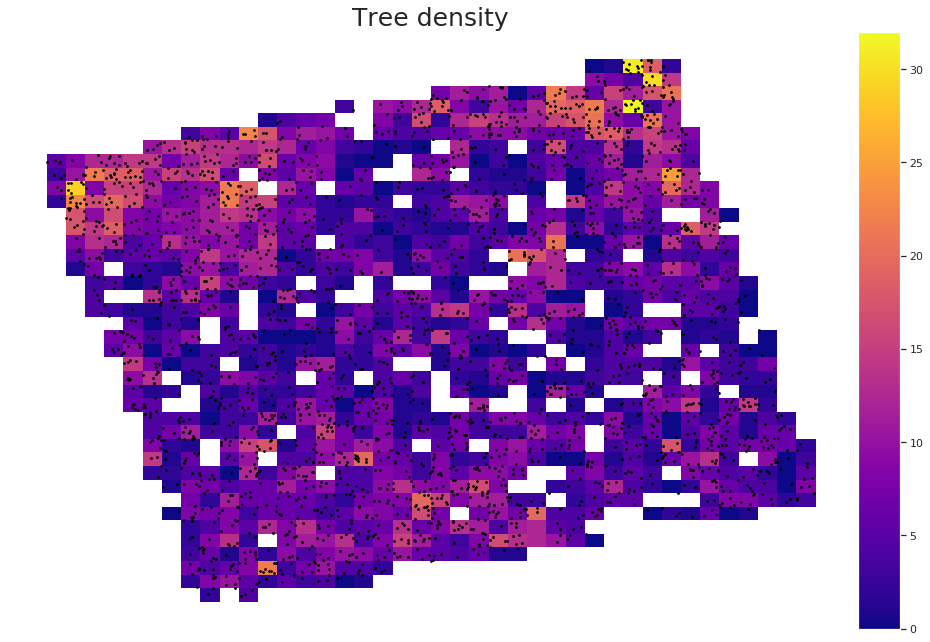
\includegraphics[scale=.45]{../figures/ESDA_density.png}
\caption{Gridded plot of tree density at the 5 meter scale.}
\label{ESDA_density} 
\end{figure}

%% ESDA HEIGHT
\begin{figure}[H]
\centering
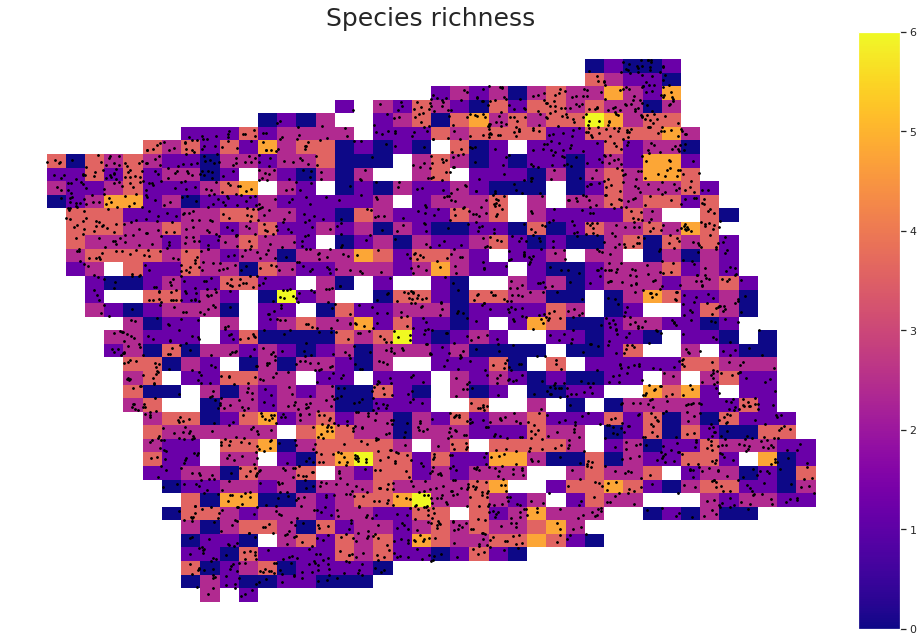
\includegraphics[scale=.45]{../figures/ESDA_richness.png}
\caption{Gridded plot of species richness at the 5 meter scale.}
\label{ESDA_richness} 
\end{figure}

%% ESDA DBH
\begin{figure}[H]
\centering
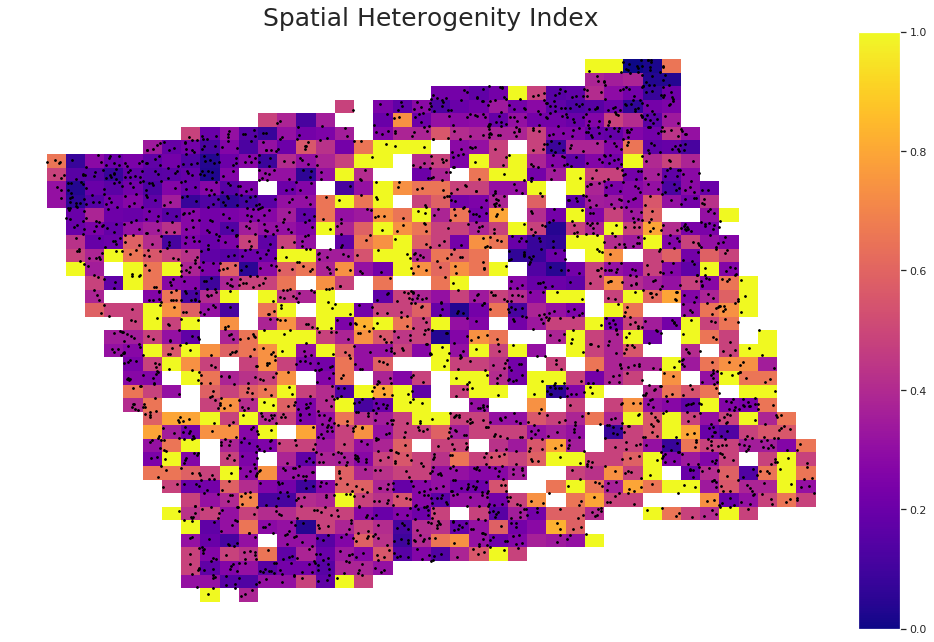
\includegraphics[scale=.45]{../figures/ESDA_shi.png}
\caption{Gridded plot of spatial heterogeneity at the 5 meter scale.}
\label{ESDA_shi} 
\end{figure}


%%%%%%%%%%%%%%%%%%%%%%%%%%%%%%%%%%%%%%%%%%%%%%%%%%%
%%%%%%%%%%%%%%%%%%%%%%%%%%%%%%%%%%%%%%%%%%%%%%%%%%%

\subsection{GWR and MGWR}


%% GWR_intercept
\begin{figure}[H]
\centering
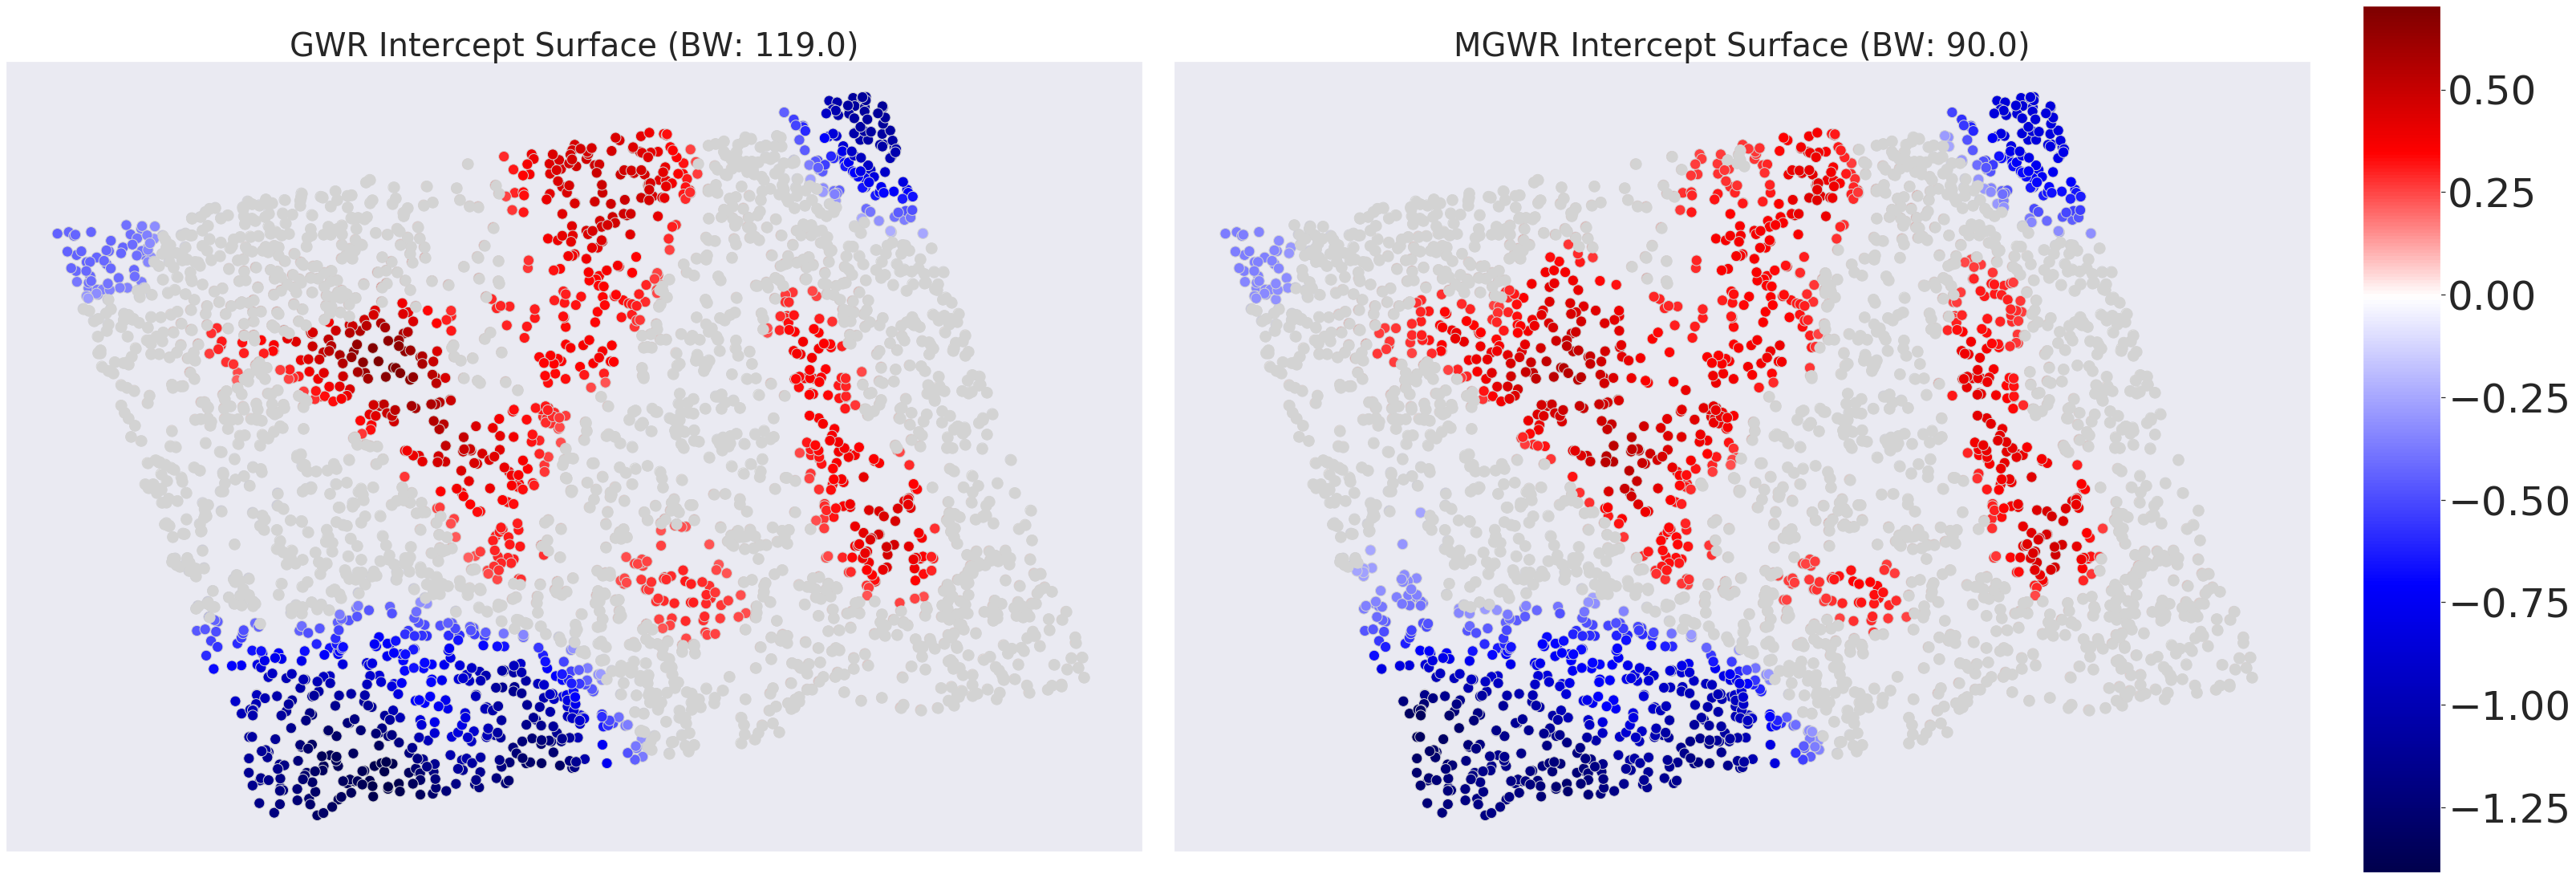
\includegraphics[scale=.13]{../figures/GWR_intercept.png}
\caption{GWR and MGWR intercept surfaces.  Colored points are significant at the 95\% confidence level.}
\label{GWR_intercept} 
\end{figure}


%% GWR_height
\begin{figure}[H]
\centering
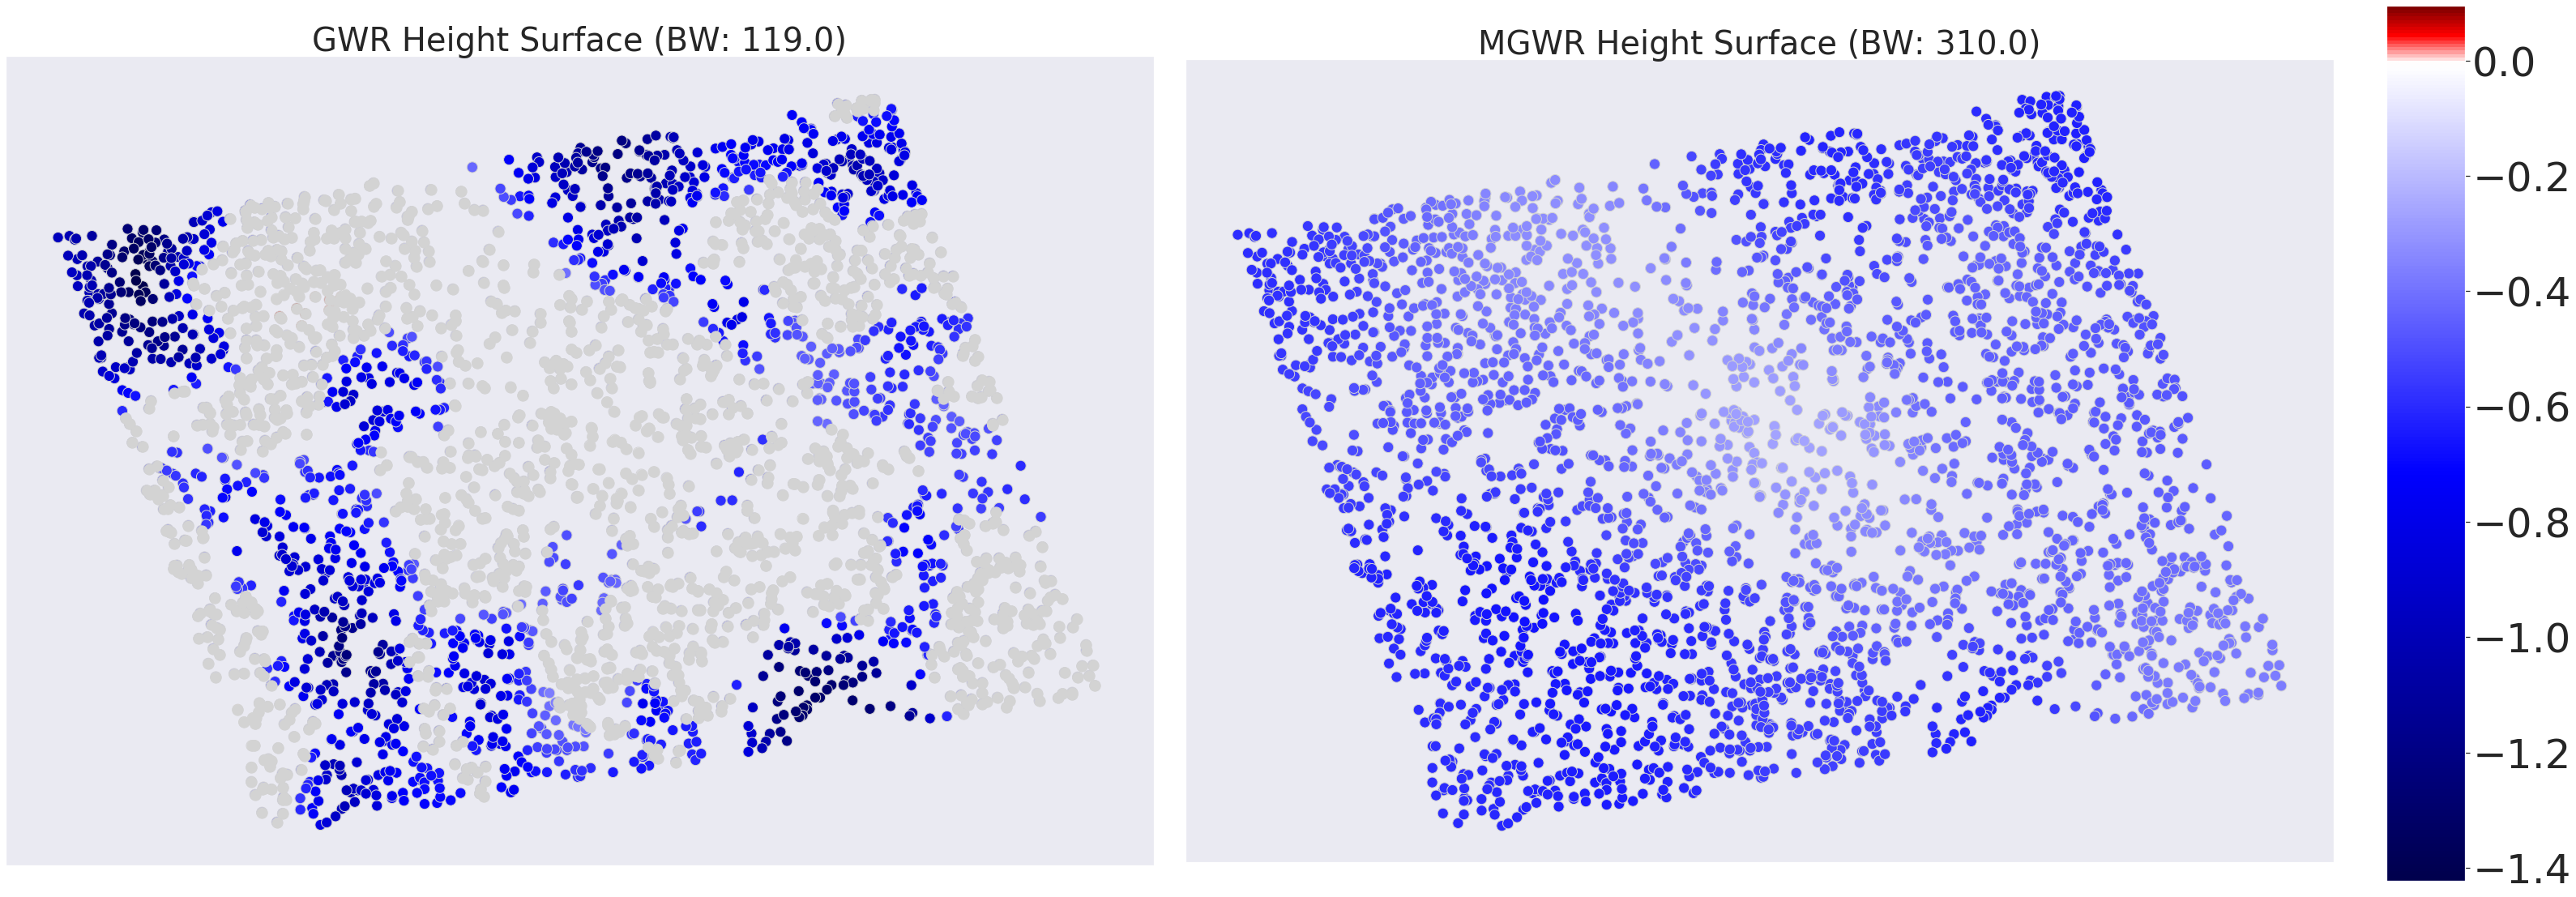
\includegraphics[scale=.13]{../figures/GWR_height.png}
\caption{GWR and MGWR coefficient surfaces for height.  Colored points are significant at the 95\% confidence level.}
\label{GWR_height} 
\end{figure}


%% GWR_height
\begin{figure}[H]
\centering
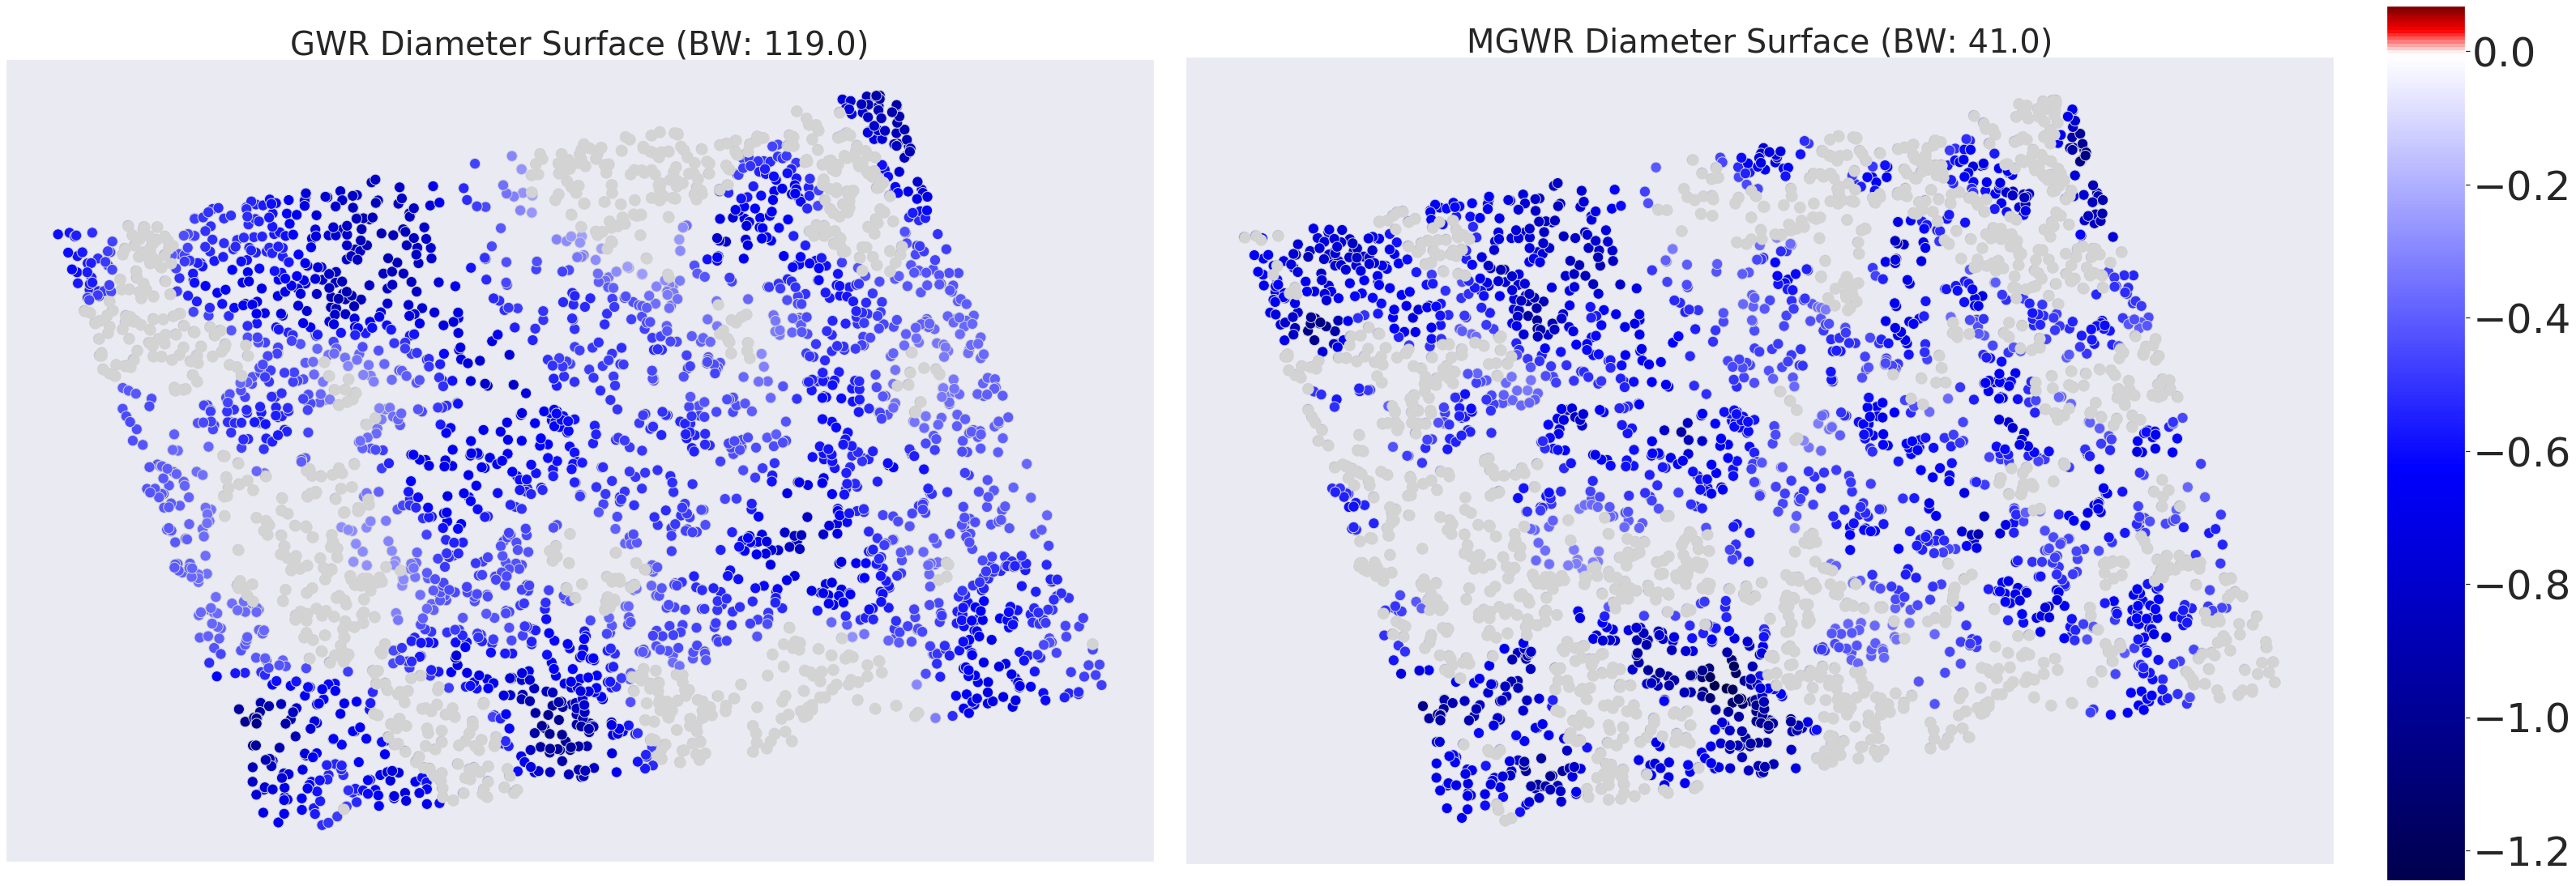
\includegraphics[scale=.13]{../figures/GWR_dbh.png}
\caption{GWR and MGWR coefficient surfaces for diameter.  Colored points are significant at the 95\% confidence level.}
\label{GWR_height} 
\end{figure}


%%%%%%%%%%%%%%%%%%%%%%%%%%%%%%%%

%% GWR_dbh
\begin{figure}[H]
\centering
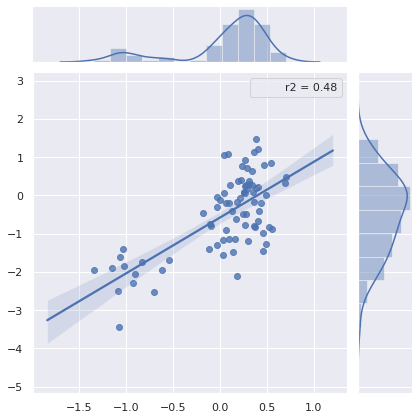
\includegraphics[scale=.65]{../figures/ModelComparison_Cnpy=1.png}
\caption{Scatter plot of the OLS model residuals vs the GWR intercept term, for super-dominant trees.}
\label{ModelComparison_Cnpy1} 
\end{figure}

%% GWR_dbh
\begin{figure}[H]
\centering
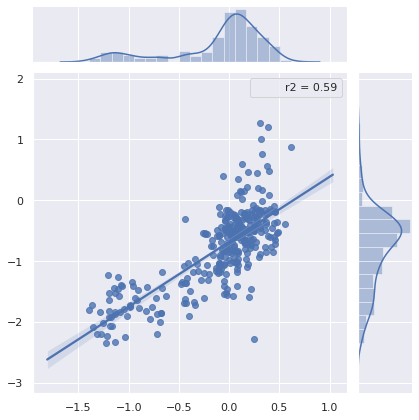
\includegraphics[scale=.65]{../figures/ModelComparison_Cnpy=2.png}
\caption{Scatter plot of the OLS model residuals vs the GWR intercept term, for dominant trees.}
\label{ModelComparison_Cnpy2} 
\end{figure}

%% GWR_dbh
\begin{figure}[H]
\centering
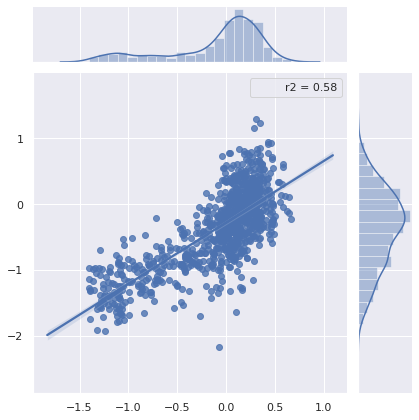
\includegraphics[scale=.65]{../figures/ModelComparison_Cnpy=3.png}
\caption{Scatter plot of the OLS model residuals vs the GWR intercept term, for co-dominant trees.}
\label{ModelComparison_Cnpy3} 
\end{figure}

%% GWR_dbh
\begin{figure}[H]
\centering
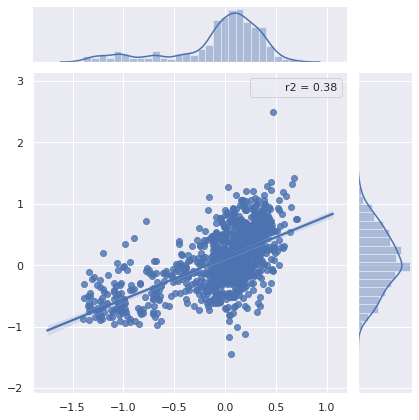
\includegraphics[scale=.65]{../figures/ModelComparison_Cnpy=4.png}
\caption{Scatter plot of the OLS model residuals vs the GWR intercept term, for intermediate trees.}
\label{ModelComparison_Cnpy4} 
\end{figure}

%% GWR_dbh
\begin{figure}[H]
\centering
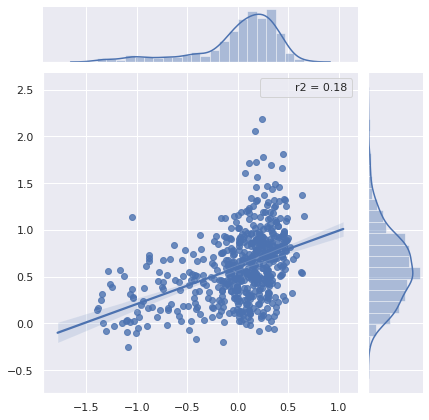
\includegraphics[scale=.65]{../figures/ModelComparison_Cnpy=5.png}
\caption{Scatter plot of the OLS model residuals vs the GWR intercept term, for over-topped trees.}
\label{ModelComparison_Cnpy5} 
\end{figure}

%% GWR_dbh
\begin{figure}[H]
\centering
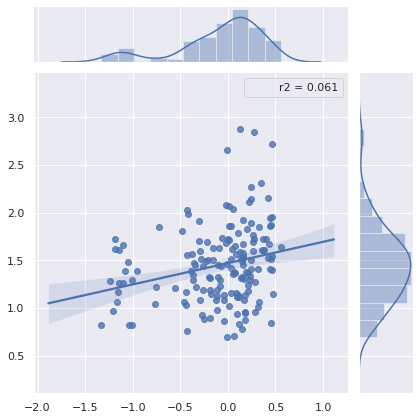
\includegraphics[scale=.65]{../figures/ModelComparison_Cnpy=6.png}
\caption{Scatter plot of the OLS model residuals vs the GWR intercept term, for suppressed trees.}
\label{ModelComparison_Cnpy6} 
\end{figure}




\newpage
\bibliographystyle{apa}
\bibliography{final_paper.bib}



\end{document}
